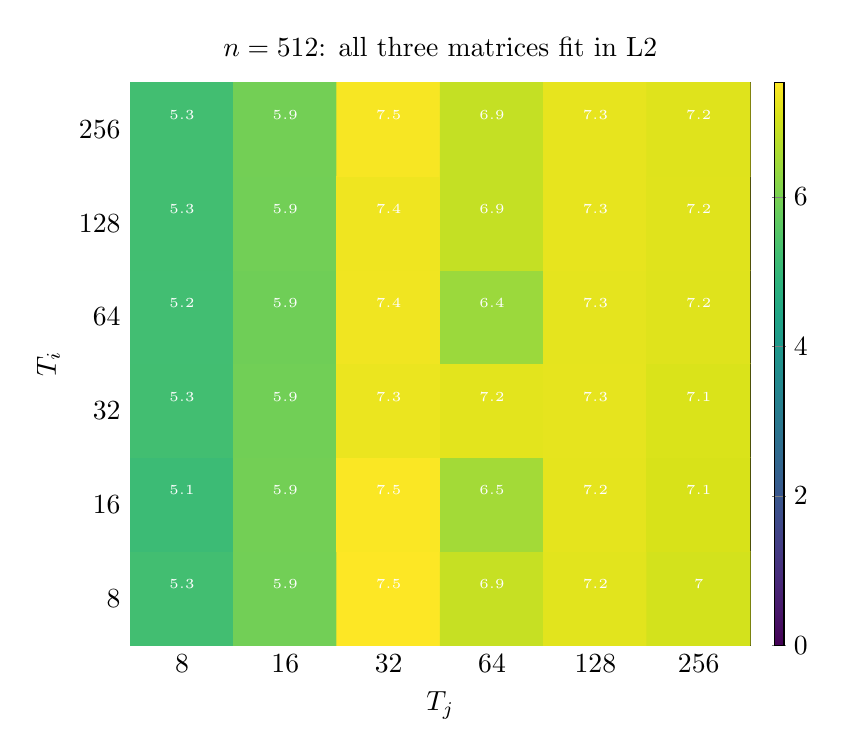
\begin{tikzpicture}
\begin{axis}[width=0.78\linewidth, height=0.72\linewidth, view={0}{90}, colorbar, colorbar style={width=0.12cm, ytick={0,2,4,6,8}, ylabel={}}, colormap/viridis, xlabel={$T_j$}, ylabel={$T_i$}, title={$n=512$: all three matrices fit in L2},
  xtick={0,...,5}, xticklabels={8,16,32,64,128,256}, ytick={0,...,5}, yticklabels={8,16,32,64,128,256},
  enlargelimits=false, point meta min=0, nodes near coords={\pgfmathprintnumber[precision=1]{\pgfplotspointmeta}}, nodes near coords style={font=\tiny, white}]
\addplot[matrix plot*, point meta=explicit, mesh/cols=6] coordinates {
(0,0) [5.25]
(1,0) [5.92]
(2,0) [7.53]
(3,0) [6.89]
(4,0) [7.21]
(5,0) [7.04]
(0,1) [5.14]
(1,1) [5.93]
(2,1) [7.49]
(3,1) [6.50]
(4,1) [7.24]
(5,1) [7.09]
(0,2) [5.25]
(1,2) [5.91]
(2,2) [7.32]
(3,2) [7.22]
(4,2) [7.26]
(5,2) [7.12]
(0,3) [5.24]
(1,3) [5.89]
(2,3) [7.37]
(3,3) [6.41]
(4,3) [7.25]
(5,3) [7.18]
(0,4) [5.25]
(1,4) [5.92]
(2,4) [7.36]
(3,4) [6.87]
(4,4) [7.27]
(5,4) [7.19]
(0,5) [5.25]
(1,5) [5.93]
(2,5) [7.46]
(3,5) [6.87]
(4,5) [7.27]
(5,5) [7.18]
};
\end{axis}
\end{tikzpicture}